\section{はじめに}

この文章は、\cite{grisetti2010}などのチュートリアルを見ても数式の細かいところが分からない
graph-based SLAMについて、
実際の計算方法を細かく解説するためのものです。

\section{問題}

%対向二輪型(その場で回転できるロボット)で、
平面上を移動し、向きを持ち、カメラでランドマーク観測ができるロボットで
graph-based SLAMを実行する方法を考える。ランドマークは環境にいくつか存在し、
ロボットからは互いに識別でき、距離と見える方角が観測できる。
また、ランドマークには向きがあり、世界座標系でどの方角を向いているのかも
ロボットから観測できるものと仮定する。

\subsection{ロボットの姿勢と座標系}

世界座標系$\Sigma_\text{w}$におけるロボットの姿勢(位置と向き)を
\begin{align}
	\V{x} =
	\begin{bmatrix}
		x \\ y \\ \theta
	\end{bmatrix}
\end{align}
で表す。また、$[x\ y]^T$を原点として、$X$軸が世界座標系で$\theta$の方向を向いているロボット座標系
$\Sigma_\text{r}$を考える。これらの関係を図\ref{fig:coordinate}に示す。

\begin{figure}[htbp]
	\begin{center}
		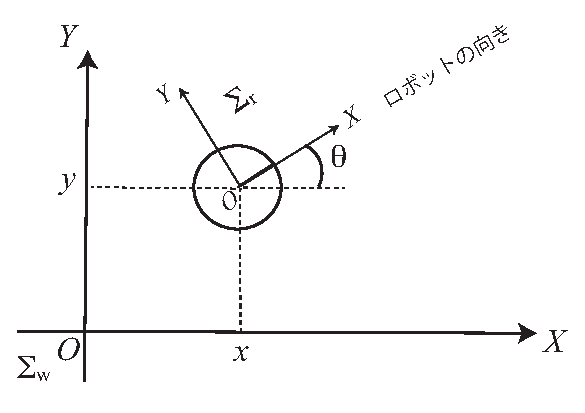
\includegraphics[width=0.5\linewidth]{./figs/coordinate.eps}
		\caption{世界座標系とロボットの姿勢}
		\label{fig:coordinate}
	\end{center}
\end{figure}

%\subsection{ロボットの運動}

離散的な時刻$t = 0,1,2,\dots,T$を考える。
時刻$t$における世界座標系でのロボットの姿勢を$\V{x}_t$で表す。
%ロボットは1単位時間で、ロボット座標系の$X$軸方向に前進した後にその場で回転することができる。
%この時の前進距離、回転角をそれぞれ$v,\omega$とする。
%また、時刻$t-1$から$t$までのこれらの量を$\V{a}_t = [v_t\ \omega_t]^T$と表す。

\subsection{観測}
